\section{Pre-training}\label{sec:pre_training}
The concept of pre-training is inspired by human beings. Thanks to an innate ability, we don’t have to learn everything from scratch. Instead, we transfer and reuse our old knowledge of what we have learned in the past to understand new knowledge and handle a variety of new tasks.

In Deep Learning, pre-training imitates the way human beings process new knowledge. That is: using model parameters of tasks that have been learned before to initialize the model parameters of new tasks. In this way, the old knowledge helps new models successfully perform new tasks from old experience instead of from scratch.

For all these reasons, we performed pre-training on both the two branches of the previously described (\vref{sec:architecture}) neural network architecture.

\subsection{Autoencoder}

In this section, we are going to define the architecture of the CNN and LSTM autoencoders we used to pre-train the two branches of the network used in this experiment.

Autoencoders are an unsupervised artificial neural network class that learn how to efficiently encode an input vector, creating a compressed but meaningful "latent space" representation of it, in order to reconstruct it back obtaining a vector that is as close as possible to the original one. Furthermore, by design, autoencoders reduce data dimensions by learning how to ignore the noise in the data, thus they serve as very good de-noising tools.

They generally consists of four components:
\begin{description}
    \item[Encoder:] one or more stacked neural network layers $e_0, ..., e_h$ composing a function $f$, in which the model learns how to reduce the input dimensions and compress the input pattern $x$ into an encoded representation $f(x)$.
    
    \item[Bottleneck:]: the last encoder layer $e_h$, containing the compressed representation $f(x)$.
    
    \item[Decoder:] one or more stacked neural network layers $d_1, ..., d_r$ (usually, the decoder is built in a mirror-like fashion with respect to the encoder, so $r = h$, $d_1$ has the same parameters as $l_h$, $d_2$ has the same as $l_{h-1}$ and so on). These layers compose a decoder function $g$, in which the model learns how to reconstruct the original input data from the encoded representation $f(x)$ in such a way that $g(f(x))$ is as close to the original input $x$ as possible.
    
    \item[Reconstruction Loss:] exactly as in regular neural networks, autoencoders are trained with an optimization algorithm in order to minimize a loss function $J$; the only difference here is that in autoencoders the loss represents the distance between input and reconstructed output:
    $$
    J = \frac{1}{|D|} \sum_{x \in D} L(x, \hat{x}) \text{, }
    $$
    where $\hat{x}$ is the reconstruction of the network on input $x$.
    
    Often, regularization techniques such as dropout \cite{dropout} or regularization terms added to the autoencoder loss functions are used, since this has the double advantage of reducing overfitting and make the learned representation sparse, which is more suitable for different tasks other than input reconstruction, which is exactly the aim of pre-training. Another way to make the learned representation sparse is to add penalization term to the loss, based on the activation value of the bottleneck neurons:
    
    $$J = \frac{1}{|D|} \sum_{x \in D} L(x, \hat{x}) + \lambda \sum_i a^{(h)}_i \text{, }$$
    where $a^{(h)}_i$ is the activation value of the $i$-th neuron of the bottleneck.
    
    By virtue of the above, dropout and activation penalization techniques were applied to the autoencoders created for the pre-training phase of this study to make the learned audio representation as sparse as possible.
\end{description}

\subsubsection{CNN Autoencoder}\label{subsec:cnnautoencoder}
The autoencoder used to pre-train the parameters of the convolutional branch of the RecConvSiameseNet uses log-scaled Mel spectrum features extracted from each speakers'audio as input. For SI, it is important to derive features that contain the vocal characteristics of the speaker, and indeed the aim here is to provide the network with a global overview of high-level features of the audio, in contrast to the LSTM branch that aims to extract temporal-wise features.

\begin{figure}
	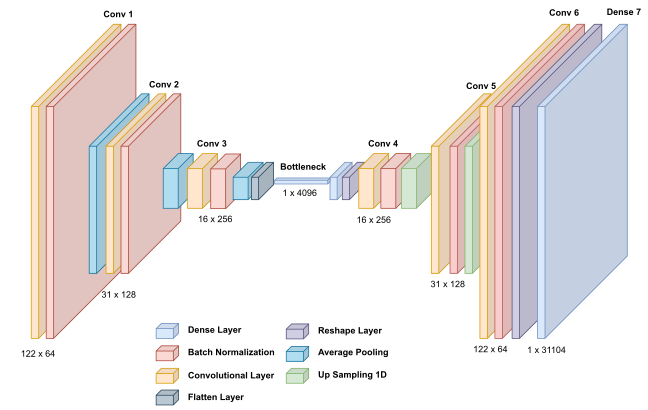
\includegraphics[width=0.5\textwidth]{images/cnn_autoencoder}
	\caption{CNN Autoencoder}
	\label{fig:cnn_autoencoder}
\end{figure}

SGD (Stochastic Gradient Descent) algorithm has been used with a learning rate of $\eta = 0.05$ to train the autoencoder for 1500 epochs with a batch size of 100 (\vref{fig:cnn_autoencoder_loss}), clipping the $L_2$ norm of the gradient to 1 and the value to of weight gradient to 0.5, in order to reduce overfitting and avoid gradient exploding.

Furthermore, as briefly mentioned before, a dropout rate of 0.5 has been applied alongside bottleneck activity regularization to prevent overfitting and make the learned data representations as sparse as possible.

\begin{figure}
	\includegraphics[width=0.5\textwidth]{images/cnn_autoencoder_graph.png}
	\caption{CNN Autoencoder Train/Validation Loss over  the first 500 epochs.}
	\label{fig:cnn_autoencoder_loss}
\end{figure}

Looking at the structure in detail, we will explore layer by layer the structure of the encoder and decoder (excluding dropout layers).

Our model's encoder consists of $3$ convolutional layers with an increasing number of filters, always followed by a batch normalization layer and by an average pooling layer that downsamples the input representation by taking the average value over the window defined by the pool size. The complete set of the encoder parameters is reported in table \vref{tab:cnn_encoder}.

\begin{footnotesize}
	\begin{table}
		\centering
		\caption{Parameters of CNN Encoder}
		\label{tab:cnn_encoder}
		\begin{tabularx}{0.5\textwidth}{XXr}%lMr
			\toprule
			\textbf{Layer Type} & \textbf{Parameters}                                                                   & \textbf{Shape} \\
			\midrule
			Input               &                                                                                       & (1, 243, 128)  \\
			Conv 1D             & \shortstack{\\ Filters, kernel, stride \\(64, 7, 2) \vphantom{space} }                & (122, 64)      \\[0.25cm]
			Batch Normalization & Features = 64                                                                         & (122, 64)      \\[0.25cm]
			Average Pooling     & Pool size = 2                                                                         & (61, 64)       \\[0.25cm] 
			Conv 1D             & \shortstack{\\ Filters, kernel, stride \\(128, 5, 2) \vphantom{space} }               & (31, 128)      \\[0.25cm]
			Batch Normalization & Features = 128                                                                        & (31, 128)      \\[0.25cm]
			Average Pooling     & Pool size = 2                                                                         & (16, 128)      \\[0.25cm]
			Conv 1D             & \shortstack{\\ Filters, kernel, stride \\(256, 5, 1) \vphantom{space} }               & (16, 256)      \\[0.25cm]
			Batch Normalization & Features = 128                                                                        & (16, 256)      \\[0.25cm]
			Average Pooling     & Pool size = 2                                                                         & (8, 256)       \\[0.25cm]
			Flatten Dense       &                                                                                       & (1, 4096)      \\
			\bottomrule
		\end{tabularx}
	\end{table}
\end{footnotesize}

The decoder is very similar to the encoder, but in reverse order, as it reconstructs the encoder’s input based on encoder’s output.

In order to match the dimension of the input, three transposed convolutional layers are needed
in the decoder in combination with upsampling layers that repeats each temporal step $r$ times along the time axis, upscaling the dimension of the reconstructed pattern, and a final triplet composed of reshape, dense and reshape layers. Decoder parameters are reported in Table \vref{tab:cnn_decoder}, while complete model architecture can be visualized in Figure \vref{fig:cnn_autoencoder}.

\begin{footnotesize}
	\begin{table}
		\centering
		\caption{Parameters of CNN Decoder}
		\label{tab:cnn_decoder}
		\begin{tabularx}{0.5\textwidth}{XXr}%lMr
			\toprule
			\textbf{Layer Type} & \textbf{Parameters}                                                                   & \textbf{Shape}    \\
			\midrule
			Dense               &                                                                         				& (1, 4096)         \\[0.25cm]
			Reshape             &                                                                                       & (16, 256)         \\[0.25cm]
			Conv 1D Transpose   & \shortstack{\\ Filters, kernel, stride \\(256, 5, 1) \vphantom{space} }               & (16, 256)         \\[0.25cm]
			Batch Normalization & Features = 256                                                                        & (16, 256)         \\[0.25cm]
			Up Sampling 1D      & Size = 2                                                                              & (32, 256)         \\[0.25cm]
			Conv 1D Transpose   & \shortstack{\\ Filters, kernel, stride \\(128, 5, 2) \vphantom{space} }               & (64, 128)         \\[0.25cm]
			Batch Normalization & Features = 128                                                                        & (64, 128)         \\[0.25cm]
			Up Sampling 1D      & Size = 2                                                                              & (128, 128)        \\[0.25cm]
			Conv 1D Transpose   & \shortstack{\\ Filters, kernel, stride \\(64, 7, 2) \vphantom{space} }                & (256, 64)         \\[0.25cm]
			Batch Normalization & Pool size = 2                                                                         & (256, 64)         \\[0.25cm]
			Reshape             &                                                                                       & (1, 16384)        \\[0.25cm]
			Dense               &                                                                          				& (1, 31104)        \\[0.25cm]
			Reshape             &                                                                                       & (1, 243, 128)     \\
			\bottomrule
		\end{tabularx}
		
	\end{table}
	
\end{footnotesize}

\subsubsection{LSTM Autoencoder}\label{subsec:recautoencoder}
The autoencoder used to pre-train the parameters of the recurrent branch of the RecConvSiameseNet takes MFCCs \& deltas features extracted from each speakers'audio as input, processing the frames one-by-one. The aim here is to extract temporal-wise features from the long-term and short-term relationships between the MFCC \& deltas frames, thanks to the memory capabilities of LSTM layers.

\begin{figure}
	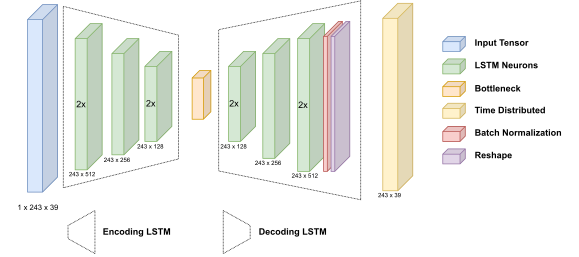
\includegraphics[width=0.5\textwidth]{images/lstm_autoencoder}
	\caption{LSTM Autoencoder}
	\label{fig:lstm_autoencoder}
\end{figure}

Adadelta algorithm has been used with a learning rate of $\eta = 1$ (as suggested by the original paper \cite{adadelta}), $\rho=0.95$ and $\epsilon=10^{-8}$ to train the LSTM autoencoder for 1000 epochs with a batch size of 200~(\vref{fig:lstm_autoencoder_loss}). 

Similar to what we have seen with the convolutional autoencoder, bottleneck activity regularization has been applied, in order to reduce overfitting and make the learned data representations as sparse as possible.

\begin{figure}
	\includegraphics[scale=0.5]{images/lstm_autoencoder_graph.png}
	\caption{LSTM Autoencoder Train/Validation Loss over the first 500 epochs.}
	\label{fig:lstm_autoencoder_loss}
\end{figure}

Diving into the architecture, encoder consists of four LSTM layers with an increasing number of units and a bottleneck of 128 units, as seen in Table~\vref{tab:lstm_encoder}.

\begin{footnotesize}
	\begin{table}
		\centering
		\caption{Parameters of LSTM Encoder}
		\label{tab:lstm_encoder}
		\begin{tabularx}{0.5\textwidth}{XXr}%lMr
			\toprule
			\textbf{Layer Type} & \textbf{Parameters}                                                                   & \textbf{Shape}    \\
			\midrule 
			LSTM               	& Units = 512	                                                                        & (243, 512)        \\[0.25cm] 
			LSTM               	& Units = 512	                                                                        & (243, 512)         \\[0.25cm] 
			LSTM               	& Units = 256	                                                                        & (243, 256)         \\[0.25cm]
			LSTM               	& Units = 128	                                                                        & (243, 128)         \\[0.25cm] 
			Bottleneck          & Dimension = 128	                                                                    &      \\ 
			\bottomrule
		\end{tabularx}
		
	\end{table}
	
\end{footnotesize}

As in the convolutional autoencoder, the decoder is built to a mirrored fashion with respect to the encoder, as we can see in the Table~\vref{tab:lstm_decoder} showing the decoder parameters. A reshape and a time distributed dense layer have been added at the end of the architecture in order to reconstruct the same shape as the fed input. The full LSTM autoencoder architecture is seen in Figure~\vref{fig:lstm_autoencoder}.

\begin{footnotesize}
	\begin{table}
		\centering
		\caption{Parameters of LSTM Decoder}
		\label{tab:lstm_decoder}
		\begin{tabularx}{0.5\textwidth}{XXr}
			\toprule
			\textbf{Layer Type} & \textbf{Parameters}                                                                   & \textbf{Shape}     \\ 
			\midrule
			LSTM               	& Units = 128	                                                                        & (243, 128)         \\[0.25cm] 
			LSTM               	& Units = 256	                                                                        & (243, 256)         \\[0.25cm] 
			LSTM               	& Units = 512	                                                                        & (243, 512)         \\[0.25cm]
			LSTM               	& Units = 512	                                                                        & (243, 512)         \\[0.25cm] 
			Batch Normalization & Features = 1024	                                                                    & (243, 1024)        \\[0.25cm]  
			Time Distributed (Dense)  	& Units = 39				                                                    & (243, 39)          \\
			\bottomrule
		\end{tabularx}
	\end{table}
\end{footnotesize}

\subsubsection{Evaluation Metrics}
Table \vref{tab:training_values_in_known_methods} illustrates the error rate analysis of the proposed autoencoders compared with some existing algorithms, such as the multiobjective evolutionary optimization algorithm~\cite{c4}, other deep convolutional and recurrent autoencoder neural networks~\cite{c5}, continual learning algorithms~\cite{c6}, enhancement parameter with a genetic algorithm~\cite{c7}, DTW~\cite{c8} and HHSAE-ASR~\cite{c9}. 

There are many possible metrics to evaluate the performances of autoencoders, but the general idea is to evaluate the reconstruction error like a distance between input and reconstructed input.

\paragraph{Mean Absolute Error}
$\mse$ evaluates the absolute distance of the observations (entries of the dataset) to the predictions on a regression, taking the average over all observations. We use the absolute value of the distances so that negative errors are accounted properly:

$$
\mae = \frac{1}{n} \sum_{i=1}^{n} \abs*{ \, \,\, y_{i}^{\text {real }}-y_{i}^{\text {pred }}}
$$

\paragraph{Mean Squared Error}
Another way to deal with negative values is by squaring the distance, so that the results are positive. This is done by the $\mse$, and higher errors (or distances) weight more in the metric than lower ones, due to the nature of the power function:

$$
\mse=\frac{1}{n} \sum_{i=1}^{n}\left(y_{i}^{\text {real }}-y_{i}^{\text {pred }}\right)^{2}
$$

\paragraph{Root Mean Squared Error}
A backlash in $\mse$ is the fact that the unit of the metric is also squared, so if the model tries to predict price in $US\$$, the $\mse$ will yield a number with unit $(US\$)^2$ which does not make sense. $\rmse$ is used then to return the $\mse$ error to the original unit by taking the square root of it, while maintaining the property of penalizing higher errors:

$$
\rmse=\sqrt{\mse}=\sqrt{\frac{1}{n} \sum_{i=1}^{n}\left(y_{i}^{\text {real }}-y_{i}^{p r e d}\right)^{2}}
$$

\paragraph{R$^2$}
It is a statistical measure in a regression model that determines the proportion of variance in the dependent variable that can be explained by the independent variable. In other words, r-squared shows how well the the regression model fits the data.
Denoting with $\bar{y}$ the mean of the real label values, and with $y_i$, $f_i$ the real label value and model prediction on $i$-th instance, respectively:
$$
\bar{y}=\frac{1}{n} \sum_{i=1}^{n} y_{i} \text{, }
$$
then the variability of the data set can be measured with two sums of squares formulas:
\begin{itemize}
	\item the sum of squares of residuals, also called the residual sum of squares:
	$$
	S S_{\text {res }}=\sum_{i}\left(y_{i}-f_{i}\right)^{2}=\sum_{i} e_{i}^{2}
	$$
	
	\item The total sum of squares (proportional to the variance of the data):
	$$
	S S_{\text {tot }}=\sum_{i}\left(y_{i}-\bar{y}\right)^{2}
	$$
\end{itemize}
That being said, the most general definition of the coefficient of determination is:

$$
R^{2}=1-\frac{S S_{\mathrm{res}}}{S S_{\mathrm{tot}}}
$$
In the best case, the modeled values exactly match the observed values, which results in $SS_{res} = 0$ and $R^2 = 1$. A baseline model, which always predicts $\bar{y}$, will have $R^2 = 0$. Models that have worse predictions than this baseline will have a negative $R^2$.

\paragraph{Analysis}
$\mse$ and $\rmse$ are very useful in understanding whether outliers generate noise in the prediction, while MAE is slightly less affected by them, so using the one or the other is a fair trade-off.\\

Optimising for $\mse$ for example, means that the generated output values are symmetrically close to the input values, meaning that an higher-than-real value is penalised by the same amount as an equally lowered one.

As for the obtained results shown in \vref{tab:training_values_in_known_methods}, it's worth noting that although the $\mae$ and $\rmse$ values of our autoencoders are particularly high if compared to the others mentioned above, this is fairly intentional and due both to the choice of not normalizing the input data, and to the applying of heavy regularization in order to make the learned weights and representations as sparse as possible and suited for usage in classification task.
Nevertheless, it's also interesting to note how both autoencoders achieve good $R^2$ values, which are satisfactorily high in the case of the convolutional one and very high in the case of the recurrent one.

\begin{footnotesize}
	\begin{table}
		\centering
		\caption{training values Error rate in Speech Processing.}
		\label{tab:training_values_in_known_methods}
		\begin{tabularx}{0.5\textwidth}{Xrrr}
			\toprule
			\textbf{Methods} 		& \shortstack{\textbf{MAE}}    	& \shortstack{\textbf{RMSE}} & \shortstack{\textbf{$R^2$}}      \\
			\midrule
			Multiobjective evolutionary\\ optimisation algorithm \cite{c4}  &N/A           & 1.43          &N/A\\
			Deep convolution\\encoder and LSTM-RNN \cite{c5}          	    &N/A           & 1.38          &N/A\\[0.25cm]
			Continual learning algorithms \cite{c6} 					    &N/A           & 1.25          &N/A\\[0.25cm]
			Genetic algorithm \cite{c7}									    &N/A           & 1.14          &N/A\\[0.25cm]
			MFCC and DTW \cite{c8}										    &N/A           & 1.12          &N/A\\[0.25cm]	
			HHSAE-ASR \cite{c9}												&N/A           & 1.087         &N/A\\[0.25cm]
			Convolutional Autoencoder\\with Mel Spectrogram				    &4.570         &6.227		   &0.8464\\[0.25cm]	
			LSTM Autoencoder\\with MFCC									    &1.796		   &2.885		   &0.9983\\
			\bottomrule
		\end{tabularx}	
	\end{table}
\end{footnotesize}
